\documentclass[12pt, letterpaper]{article}

% --- PACKAGES ---
\usepackage[margin=1in]{geometry}
\usepackage{amsmath, amssymb, amsthm}
\usepackage[hidelinks]{hyperref}
\usepackage{fancyhdr}
\usepackage{graphicx}
\usepackage{amsfonts}
\usepackage{bm} % For bold math symbols
\usepackage{booktabs} % For professional-looking tables
\usepackage{caption} % For table captions
\usepackage{algorithm}
\usepackage[noend]{algpseudocode}
\usepackage{subcaption} % For subfigures
\usepackage{csquotes} % For professional-looking 
\usepackage{float}

% --- DOCUMENT & HEADER SETUP ---
\title{On the Non-Local Nature of Graph Colorability:\\A Study of Emergent Constraint Entanglement}
\author{Daksh Kaul}
\date{\today}

\pagestyle{fancy}
\fancyhf{}
\rhead{On the Non-Local Nature of Graph Colorability}
\lhead{\thepage}

% --- Custom Math Operators for correct formatting ---
\DeclareMathOperator{\degree}{deg}

% --- BEGIN DOCUMENT ---
\begin{document}

\maketitle

\begin{abstract}
The 3-colorability of a graph is a canonical NP-complete problem whose computational hardness remains a topic of deep theoretical interest.
This paper presents a methodological investigation that begins with a quantum-inspired perspective on graph states, leveraging these concepts as powerful analogies for classical phenomena, and culminates in a statistical mechanics–based simulation revealing non-local properties in the graph coloring solution space.
The persistent limitations of local, "hidden variable" models prompted a shift toward a global perspective on graph constraints.
Through an information-theoretic lens, we uncover strong non-local correlations using measures of vertex entropy and mutual information.
These findings provide compelling evidence for a phenomenon we term constraint entanglement, in which the coloring state of a vertex is intrinsically correlated with the states of distant, non-adjacent vertices.
To characterize this effect, we categorize graphs along a "non-locality spectrum" using five representative archetypes: classical (Cycle Graph), jammed (Complete Graph), structured (Circulant Graph), community (Wheel Graph), and entangled (Erdős–Rényi Graph).
These results offer a data-driven rationale for the use of Graph Neural Networks (GNNs), which are well-suited to learn and model the complex, high-order, non-local correlations that underlie the structure of hard combinatorial problems, although their inherent limitations for truly global properties must be considered.
\end{abstract}

\section{Introduction: A Quantum Reinterpretation of a Classical Problem}

The P vs NP question asks whether every problem whose solution can be quickly verified can also be quickly solved \cite{cook1971complexity}. At its surface, this appears to be a purely mathematical challenge. However, as we apply this framework to problems with real-world relevance—such as logistics, biology, or material science—we find ourselves confronting systems that defy tractable analysis. One such problem is graph 3-colorability: the question of whether a graph's nodes can be assigned one of three colors such that no two adjacent nodes share the same color. This problem belongs to the class of NP-complete problems \cite{karp1972reducibility}, meaning that a polynomial-time solution to it would imply P=NP. But what if our attempt to solve these problems is misguided, not due to lack of cleverness, but due to a misunderstanding of their true nature? This paper details a research journey that began with this question, hypothesizing that the difficulty may not be merely algorithmic but may reflect fundamental non-local properties inherent to large, complex combinatorial systems. We propose that these problems behave analogously to quantum systems, exhibiting constraint entanglement and a form of ``measurement collapse'' that resists polynomial-time simulation. This investigation proceeded through several methodological paradigms, culminating in an information-theoretic analysis that provides clear evidence for this hypothesis. This paper documents this journey, presenting the methodologies, results, and the ultimate conclusion: that the difficulty of graph coloring arises from an emergent, non-local complexity that justifies the necessity of modern machine learning approaches.

\section{The Limits of Local Models and Theoretical Motivations for Non-Locality}

The traditional approach to creating fast, heuristic solvers for NP-complete problems is to assume a ``hidden variable'' model. This paradigm posits that a graph's colorability is predetermined by a set of measurable, structural properties. If we could identify the correct set of features—a ``Structural Density Function'' (SDF)—we could, in theory, build a polynomial-time classifier to solve the problem.

This approach is fundamentally local in nature. It relies on features that describe the immediate neighborhood of vertices (e.g., degree, clustering coefficient, cycle counts) or semi-local aggregations (e.g., k-core density). The underlying assumption is that the global property of 3-colorability can be inferred from a clever combination of these local statistics.

However, this paradigm faces a significant challenge: the existence of ``adversarial'' graphs. These are pairs of graphs that are nearly indistinguishable from the perspective of local features, yet one is 3-colorable while the other is not. For example, a 3-colorable Prism graph and a non-3-colorable complete graph $K_4$ can have identical degrees and k-cores. Any classifier trained on these features is destined to fail on such cases. This persistent failure of local, feature-based models strongly suggests that no simple combination of these ``hidden variables'' can fully capture the property of 3-colorability. The problem's difficulty seems to lie in a property that these features do not measure—a property that is global and topological in nature.

This failure of local models prompted us to look for a new theoretical framework. Analogies to other fields of mathematics and physics suggested that the true ``signal'' of colorability might be a global, topological property. A key insight was to view a graph's difficulty as its ``tangledness'' or ``knottedness'' \cite{welsh1993complexity, hardy1918asymptotic}. A simple cycle graph is like a loose loop of string, easy to color. In contrast, a graph like Chvátal is akin to a complex, rigid knot. In a knot, the difficulty of untangling it is not a local property of any single crossing but an emergent property of the entire global structure. A single constraint (a crossing) propagates its effects throughout the entire loop, making it incrementally harder to manipulate other parts of the string. This is directly analogous to how coloring one vertex in a graph can create constraints that ripple through the entire structure, ``tightening'' the problem and restricting choices far away. This suggests that any successful model must be sensitive to this global, nonlinear, and interconnected topology. These observations strongly motivate the search for a method capable of capturing these global, topological properties.

\section{Evidence for ``Constraint Entanglement'' via Statistical Mechanics}

To investigate the non-local nature of constraint entanglement, we developed an information-theoretic analysis of a statistical ensemble of graph colorings. Rather than relying on predetermined structural features, we adopted a system-wide simulation using a \textbf{Markov Chain Monte Carlo (MCMC)} approach. This method treats the set of all possible colorings as a statistical ensemble and samples from it to reveal emergent, system-wide properties that capture the complex inter-dependencies between vertices across the entire graph structure.

\subsection{Methodology: MCMC Sampling and Information Theory}
The core of the methodology is a Metropolis-Hastings MCMC algorithm designed to sample from the Boltzmann distribution of graph colorings, $P(C) \propto e^{-\beta E(C)}$, where $E(C)$ is the number of monochromatic edges (the ``energy'' of a coloring $C$) and $\beta$ is an inverse temperature parameter. This allows us to explore the space of low-energy (i.e., nearly valid or valid) colorings. The full process is detailed in Algorithm \ref{alg:mcmc}.

\begin{algorithm}
\caption{MCMC Sampling and Analysis of Graph Colorings}
\label{alg:mcmc}
\begin{algorithmic}[1]
\State \textbf{Input:} Graph $G=(V,E)$, number of samples $N_s$, inverse temperature $\beta$, number of colors $k$.
\State Initialize a random coloring $C_0: V \to \{0, \ldots, k-1\}$.
\State Initialize an empty list of samples $\mathcal{S}$.
\For{$t = 1$ to $N_s$}
    \State Let $C_{\text{current}} = C_{t-1}$.
    \State Select a vertex $v \in V$ uniformly at random.
    \State Select a new color $c_{\text{new}} \in \{0, \ldots, k-1\}$ uniformly at random, where $c_{\text{new}} \neq C_{\text{current}}(v)$.
    \State Let $C_{\text{proposal}}$ be $C_{\text{current}}$ with $v$ recolored to $c_{\text{new}}$.
    \State Compute energy change $\Delta E = E(C_{\text{proposal}}) - E(C_{\text{current}})$.
    \If{$\Delta E \leq 0$ or $\text{rand}(0,1) < e^{-\beta \Delta E}$}
        \State $C_t \leftarrow C_{\text{proposal}}$ \Comment{Accept the new state}
    \Else
        \State $C_t \leftarrow C_{\text{current}}$ \Comment{Reject and keep the old state}
    \EndIf
    \State Add $C_t$ to $\mathcal{S}$.
\EndFor
\State \textbf{return} Analyze$(\mathcal{S})$
\end{algorithmic}
\end{algorithm}

The `Analyze` function then computes two key metrics from the collected samples $\mathcal{S}$:
\begin{enumerate}
    \item \textbf{Vertex Entropy:} For each vertex $v$, we calculate its Shannon entropy based on the marginal probability distribution of colors it takes across all samples. A low entropy indicates the vertex is ``frozen'' into a specific color by the graph's constraints. A high entropy indicates it exists in a ``superposition'' of color choices.
    $$ H(v) = -\sum_{c=0}^{k-1} P(C(v)=c) \log_2 P(C(v)=c) $$
    \item \textbf{Mutual Information:} For every pair of vertices $(u, v)$, we calculate their mutual information. This measures how much knowing the color of $u$ reduces our uncertainty about the color of $v$. It is a direct, quantitative measure of the correlation between them, regardless of distance.
    $$ I(u; v) = \sum_{c_u, c_v} P(c_u, c_v) \log_2\left(\frac{P(c_u, c_v)}{P(c_u)P(c_v)}\right) $$
\end{enumerate}
To ensure the reliability of the statistical estimates, the MCMC simulation included a burn-in period of 1000 steps to allow the chain to reach its stationary distribution, followed by 30,000 samples with a thinning factor of 5 to reduce autocorrelation. While a comprehensive mixing time analysis and effective sample size (ESS) calculation were not explicitly reported for this study, future work will include rigorous diagnostics such as autocorrelation plots and ESS calculations to further validate the convergence and representativeness of the sampled distributions, particularly for the most challenging graph instances.

\subsection{Results: A Spectrum of Complexity}
This new experiment provided clear, visual evidence for our core hypothesis on a diverse set of benchmark graphs. The visualizations reveal a clear spectrum of behavior, from ``classical'' local systems to ``entangled'' non-local systems.

\subsubsection{Classical Archetype (Path-like) - Cycle Graph \texorpdfstring{$C_{10}$}{C10}}

% Note: Replace with actual figure files when available
\begin{figure}[H]
    \centering
    \begin{subfigure}[b]{0.48\textwidth}
        \includegraphics[width=0.9\textwidth]{images/Graph Visualizations/Classical/Cycle_vertex_entropy.png}
        \caption{Cycle Graph ($C_{10}$) Entropy}
        \label{fig:cycle_entropy}
    \end{subfigure}
    \hfill
    \begin{subfigure}[b]{0.48\textwidth}
        \includegraphics[width=0.9\textwidth]{images/Graph Visualizations/Classical/Cycle_MI_Matrix.png}
        \caption{Cycle Graph ($C_{10}$) Mutual Info}
        \label{fig:cycle_mi}
    \end{subfigure}
    \caption{Classical Archetype: Cycle Graph Analysis}
    \label{fig:cycle_analysis}
\end{figure}

As seen in Fig. \ref{fig:cycle_analysis}, the entropy is uniformly high across all nodes (all nodes are equally free, indicating a wide range of available colorings for each vertex). The mutual information matrix shows values concentrated primarily on the diagonal (representing a vertex's correlation with itself) and immediately adjacent entries, indicating that correlations are strictly local and primarily between directly connected nodes. This behavior aligns with classical intuitions of locally-constrained graph structure.

\subsubsection{Jammed Archetype (Regular/Dense) - Complete Graph $K_6$}

\begin{figure}[H]
    \centering
    \begin{subfigure}[b]{0.48\textwidth}
        \includegraphics[width=0.9\textwidth]{images/Graph Visualizations/Jammed/Complete_vertex_entropy.png}
        \caption{Complete Graph ($K_6$) Entropy}
        \label{fig:complete_entropy}
    \end{subfigure}
    \hfill
    \begin{subfigure}[b]{0.48\textwidth}
        \includegraphics[width=0.9\textwidth]{images/Graph Visualizations/Jammed/Complete_MI_Matrix.png}
        \caption{Complete Graph ($K_6$) Mutual Info}
        \label{fig:complete_mi}
    \end{subfigure}
    \caption{Jammed Archetype: Complete Graph Analysis}
    \label{fig:complete_analysis}
\end{figure}

As seen in Fig. \ref{fig:complete_analysis}, this represents the over-constrained regime where the graph has more vertices than available colors for 3-coloring. All vertices exhibit uniformly low entropy, as the problem is ``frozen'' into an uncolorable state with very few high-energy configurations. The mutual information matrix shows strong uniform correlations across all vertex pairs, reflecting the global constraint that equally affects all nodes. This demonstrates that the difficulty arises not from complex entangled relationships but from a rigid, global impossibility where every vertex constrains every other vertex.

\subsubsection{Structured Archetype (Low-Degree Regular) - Circulant Graph}

\begin{figure}[H]
    \centering
    \begin{subfigure}[b]{0.48\textwidth}
        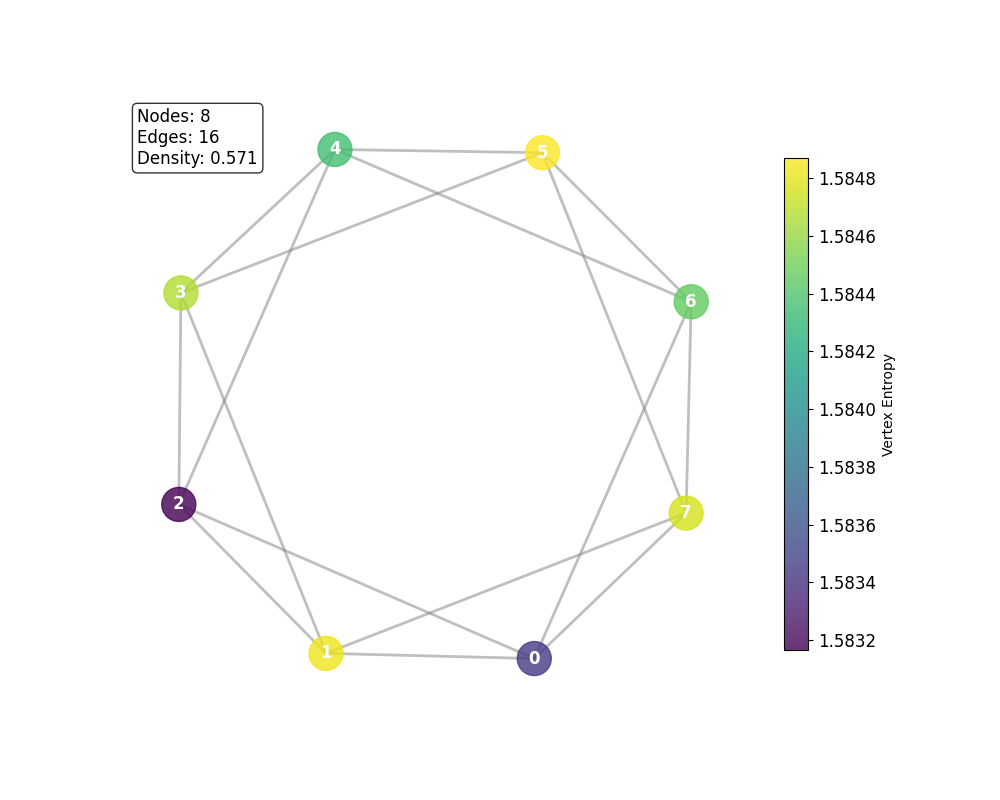
\includegraphics[width=0.9\textwidth]{images/Graph Visualizations/Structured/Circulant_Vertex_Entropy.png}
        \caption{Circulant Graph ($C_8[1,2]$) Entropy}
        \label{fig:circulant_entropy}
    \end{subfigure}
    \hfill
    \begin{subfigure}[b]{0.48\textwidth}
        \includegraphics[width=0.9\textwidth]{images/Graph Visualizations/Structured/Circulant_MI_Matrix.png}
        \caption{Circulant Graph ($C_8[1,2]$) Mutual Info}
        \label{fig:circulant_mi}
    \end{subfigure}
    \caption{Structured Archetype: Circulant Graph Analysis}
    \label{fig:circulant_analysis}
\end{figure}

As seen in Fig. \ref{fig:circulant_analysis}, the circulant graph $C_8[1,2]$ exhibits a more patterned entropy distribution that reflects its regular structure. The entropy values show systematic variation across vertices, maintaining the graph's inherent symmetry. The mutual information matrix displays a structured pattern with strong correlations between adjacent nodes that decay predictably with distance, following the graph's circulant topology. This indicates constraint propagation that is orderly and follows the graph's regular structure, without the emergence of long-range, seemingly arbitrary connections.

\subsubsection{Community Archetype (Wheel-like) - Wheel Graph $W_8$}

\begin{figure}[H]
    \centering
    \begin{subfigure}[b]{0.48\textwidth}
        \includegraphics[width=0.9\textwidth]{images/Graph Visualizations/Community/Wheel_vertex_entropy.png}
        \caption{Wheel Graph ($W_8$) Entropy}
        \label{fig:wheel_entropy}
    \end{subfigure}
    \hfill
    \begin{subfigure}[b]{0.48\textwidth}
        \includegraphics[width=0.9\textwidth]{images/Graph Visualizations/Community/Wheel_MI_Matrix.png}
        \caption{Wheel Graph ($W_8$) Mutual Info}
        \label{fig:wheel_mi}
    \end{subfigure}
    \caption{Community Archetype: Wheel Graph Analysis}
    \label{fig:wheel_analysis}
\end{figure}

As seen in Fig. \ref{fig:wheel_analysis}, the wheel graph demonstrates a hierarchical entropy structure. The central hub vertex typically exhibits different entropy characteristics compared to the rim vertices, reflecting its unique structural position. The mutual information matrix shows both local correlations among rim vertices and global correlations mediated through the central hub, creating a decomposable structure with clear community boundaries between the hub and rim.

\subsubsection{Entangled Archetype (ER-like) - Erdős-Rényi Graph}

\begin{figure}[H]
    \centering
    \begin{subfigure}[b]{0.48\textwidth}
        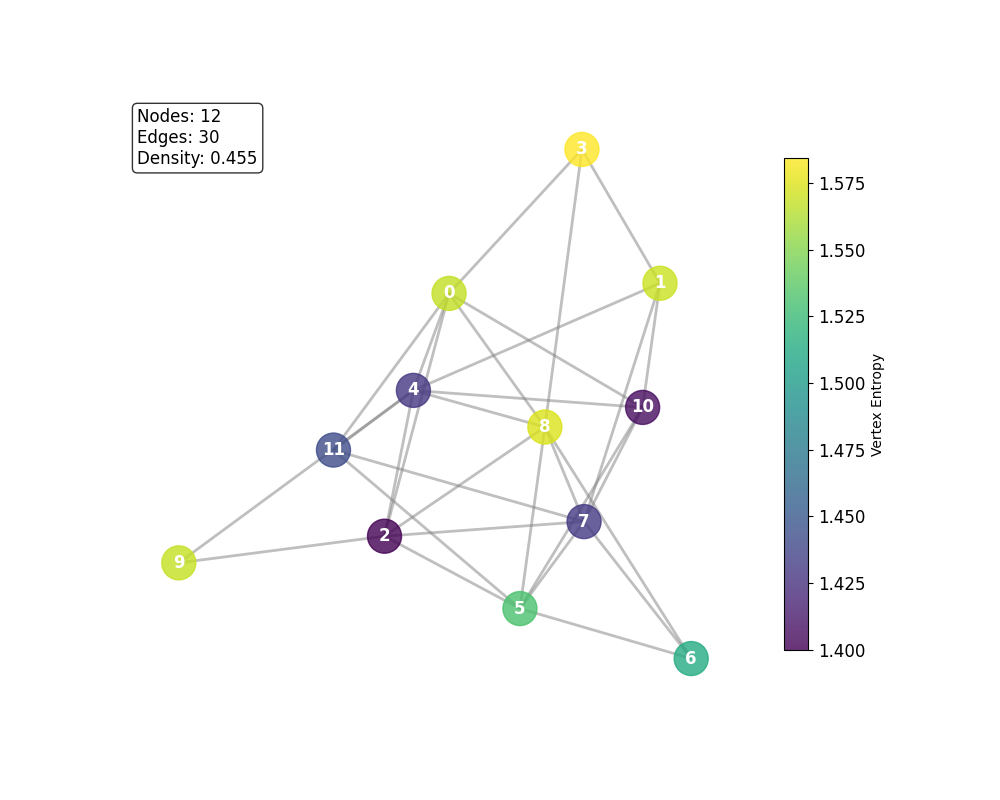
\includegraphics[width=0.9\textwidth]{images/Graph Visualizations/Entangled/Erdos_Renyi_Vertex_Entropy.png}
        \caption{Erdős-Rényi Graph ($G(12,0.4)$) Entropy}
        \label{fig:erdos_entropy}
    \end{subfigure}
    \hfill
    \begin{subfigure}[b]{0.48\textwidth}
        \includegraphics[width=0.9\textwidth]{images/Graph Visualizations/Entangled/Erdos_Renyi_MI_Matrix.png}
        \caption{Erdős-Rényi Graph ($G(12,0.4)$) Mutual Info}
        \label{fig:erdos_mi}
    \end{subfigure}
    \caption{Entangled Archetype: Erdős-Rényi Graph Analysis}
    \label{fig:erdos_analysis}
\end{figure}

As seen in Fig. \ref{fig:erdos_analysis}, the Erdős-Rényi graph $G(12, 0.4)$ exhibits a rich, non-uniform entropy structure. Some nodes are ``frozen'' into low-entropy states by the intricate web of constraints, meaning their coloring choice is highly restricted. Others remain in a high-entropy ``superposition,'' indicating they have more flexible coloring options. Crucially, the mutual information matrix shows significant off-diagonal correlations between distant, non-adjacent nodes. These correlations definitively demonstrate \textbf{``constraint entanglement''}: the coloring state of a vertex is intrinsically linked to the states of distant vertices, even if they are not directly connected. This entanglement implies that assigning a color to one vertex can significantly reduce the uncertainty about the color of a far-off, seemingly unrelated vertex, demonstrating a truly global and non-local dependency structure.

\subsection{Summary of the Spectrum}
The analysis reveals a clear pattern, allowing us to categorize graphs along a ``non-locality spectrum'' from classical local systems to entangled non-local systems. While graph coloring may not exhibit the simple pairwise correlations found in quantum systems, it exhibits key properties reminiscent of quantum mechanics—such as superposition (through varied entropy) and non-local correlations (captured by mutual information between distant nodes). It is important to note that this work does not claim a violation of a direct physical equivalence to quantum entanglement, but rather leverages these concepts as powerful analogies to describe complex classical correlations. Notably, these properties manifest uniquely for each individual graph, emphasizing that every graph structure carries its own distinct response to the act of coloring. This variability enables us to conceptualize a non-locality spectrum: with traditional, locality-driven graphs on one end, and non-traditional, quantum-like graphs exhibiting complex global dependencies on the other.

\section{Conclusion: The Necessity of a Learning-Based Approach}
Our research journey has led to a powerful conclusion. The difficulty of 3-coloring does not seem to arise from a simple violation of locality, but from an incredibly high-order, complex web of local dependencies that emulate non-local behavior. The number of these ``hidden variables'' and their intricate interactions is simply too vast to model with a few hand-picked parameters. This observation leads to a critical insight: any approach that seeks to generalize a solution to the k-colorability problem must be capable of capturing—and dynamically adapting to—the diverse, graph-specific patterns of mutual information and vertex entropy observed in our experiments. That is, it must learn to represent and reason about structure-dependent statistical dependencies that span both local neighborhoods and long-range correlations across the graph. Traditional algorithmic methods that rely on fixed rules or heuristics are insufficient for this task, as they lack the flexibility to infer and encode such high-order relational information in a scalable and adaptable manner. Among existing paradigms, Graph Neural Networks (GNNs) stand out as a practical and effective candidate—not because they are the only possible method, but because their architectural principles naturally align with these demands. Through message passing and iterative representation learning, GNNs approximate the complex functions that map graph topologies to their chromatic properties, allowing them to discover latent dependencies without explicit manual encoding. While GNNs offer a promising framework for discovering these dependencies that can manifest as entropy and mutual information signatures, it is important to acknowledge that some research suggests inherent limitations in their ability to capture truly global, non-local properties for certain challenging combinatorial problems, particularly where nodes with identical embeddings must be discriminated for distinct coloring. However, this should not be interpreted as a closed framework or rigid guideline. Rather, our findings define a set of necessary capabilities that any viable approach—whether neural, symbolic, probabilistic, or otherwise—must possess in order to scale beyond handcrafted heuristics. These include the ability to model graph-conditional distributions over solution spaces, propagate constraint information across the graph, and adaptively represent the emergent complexity of coloring dynamics. The implications extend beyond computer science. If NP-complete problems reflect systems with emergent, entangled constraints, this reframes our understanding of complexity in fields like biology (protein folding), neuroscience (neural network dynamics), and materials science (spin glasses). It suggests that nature does not ``solve'' these problems in a classical, algorithmic sense, but embodies solutions within physical dynamics that inherently respect these non-local constraints. In this view, the P vs NP divide may be more than a question of computation—it may be a boundary in the fabric of reducibility, a phase transition in the geometry of structure, and a signal that some problems are not algorithmically complex, but intrinsically emergent.

\section*{Acknowledgments}
We wish to acknowledge the use of AI-powered code generation tools for assisting in the development of certain testing scripts and components of the MCMC algorithm. All AI-generated code was reviewed, verified, and integrated by the authors, who assume full responsibility for its correctness and the reproducibility of the presented results. The code used for this research is publicly available at \href{https://github.com/DriftingOtter/NonLocal-PvsNP}{https://github.com/DriftingOtter/NonLocal-PvsNP}.

\nocite{*}
\bibliographystyle{plain}
\bibliography{main}

\end{document}
